\documentclass[11pt]{article}

%%% Load some useful packages:
%% "New" LaTeX2e graphics support.
\usepackage{graphicx}
%%	using final option to force graphics to be included even in draft mode
%\usepackage[final]{graphicx}
\usepackage{paralist} % compact lists

%% Support sub-figures.
\usepackage{subfigure}

%% Make subsubsections numbered and included in ToC
\setcounter{secnumdepth}{3}
\setcounter{tocdepth}{3}

%% Package to linebreak URLs in a sane manner.
\usepackage{url}

%% Define a new 'smallurl' style for the package that will use a smaller font.
\makeatletter
\def\url@smallurlstyle{%
  \@ifundefined{selectfont}{\def\UrlFont{\sf}}{\def\UrlFont{\small\ttfamily}}}
\makeatother
%% Now actually use the newly defined style.
\urlstyle{smallurl}

%% Make margins less ridiculous
\usepackage{fullpage}

%% Allows insertion of fixme notes for future work
\usepackage[footnote, nomargin]{fixme}

%%%% Turned off for tech report, should be turned on for research portfolio
%% Turn on double spacing
%\usepackage{setspace}
%\doublespacing

%% Make URLs clickable
\usepackage[colorlinks, bookmarks=true]{hyperref}
\usepackage[all]{hypcap}


%% Since I'm using the LaTeX Makefile that uses dvips, I need this
%% package to make URLs break nicely
\usepackage{breakurl}

\usepackage{array}

%% Adds new functionality for tables
\usepackage{tabularx}

\newcolumntype{P}[1]{>{\raggedright\arraybackslash}p{#1}}

% create a shortcut to typeset table headings
\newcommand\tabhead[1]{\small\textbf{#1}}

\usepackage{multirow}

%% Make table cross pages.
\usepackage{longtable}

\begin{document}

\title{SGSEAM Assessment Plan for Makahiki}

\author{
	 Yongwen Xu \\
\em  Collaborative Software Development Laboratory \\
\em  Department of Information and Computer Sciences \\
\em  University of Hawai'i at Manoa\\
     yxu@hawaii.edu \\
}

\date{June 2013}
\maketitle

\tableofcontents

\graphicspath{{figures/}} 
\DeclareGraphicsExtensions{.eps}


\chapter{SGSEAM Plan for Makahiki }
\label{app:makahiki-assessment-plan}

This appendix includes the SGSEAM assessment plan for Makahiki. It is the deliverable for the first step of SGSEAM when applying to Makahiki framework. It first identifies the stakeholders, determines the appropriate assessment
approaches according to the available resources, chooses assessment participants, and creates the assessment schedule.

\section{Identify SGSEAM Stakeholders in Makahiki}
The first step in SGSEAM assessment plan is to identify the stakeholders in Makahiki. \autoref{table:eval-stakeholders} listed the identified stakeholders who use the Makahiki framework. 

\begin{table}[ht!]
  \centering
  \begin{tabular}{|p{0.2\columnwidth}|p{0.4\columnwidth}|p{0.3\columnwidth}|}
    \hline
    \tabhead{Stakeholder class} &
    \tabhead{Tasks} &
    \tabhead{Role} \\
    \hline
    Player &
    Participate in the Makahiki games &
    Students living in the residential halls\\
    \hline
    System admin &
    Install Makahiki software, monitor and scale the system, backup, patch maintenance &
    IT staffs\\
    \hline
    Game designer &
    Design the content, configure suitable games and mechanics &
    Challenge organizers\\
    \hline
    Game manager &
    Manage the game during the period of game play.&
    Challenge organizers\\
    \hline
    Developer &
    Develop customization, extend and enhance the game and framework. &
    Makahiki developers \\
    \hline
  \end{tabular}
  \caption{SGSEAM Stakeholders}
  \label{table:eval-stakeholders}
\end{table}

\section {Determine SGSEAM Approaches for Makahiki}

The second step in SGSEAM plan is to determine the assessment approach. As described in SGSEAM, approaches include both  {\em in-vivo} and {\em in-vitro} assessments. The  {\em in-vivo} approaches, such as pre-post test, in-game surveys and post-hoc interviews, assess the real world instance of the game. The {\em in-vitro} approaches use in-lab experiments in a simulated environment. Different assessment approaches will have different levels of rigor or validity. When applying SGSEAM in Makahiki, I used the real world Makahiki instances as the in-vivo approaches which includes pre-post effectiveness study for player assessment, post-hoc interview for game administrator and game designer. 

In addition to real world instances assessment, I also implemented the in-vitro assessment approach using in-lab experiments. In Spring 2013, Professor Philip Johnson at the Information and Computer Science Department of University of Hawaii used Makahiki to teach a course in serious game development. The students were seniors or graduate students majoring in computer science related fields. During the course, the students installed Makahiki, designed a serious game instance with Makahiki, and developed an enhancement to the Makahiki system.
The participation was voluntary. This is considered as an in-lab experiment since they are evaluating Makahiki in a class setting and using Makahiki in the development environments.

\autoref{table:eval-approaches} lists the SGSEAM approaches that are used to assess the strengths and weaknesses of Makahiki from different stakeholders' view.

\begin{table}[ht!]
  \centering
  \begin{tabular}{|p{0.17\columnwidth}|p{0.32\columnwidth}|p{0.42\columnwidth}|}
    \hline
    \tabhead{Stakeholder}&
    \tabhead{Assessment approaches} &
    \tabhead{Expected Outcomes} \\
    \hline
    \multirow{4}{*}{Player} & Pre-post effectiveness study &
    Determine effectiveness in energy literacy and resource usage reduction \\
    \cline{2-3}
      & Self-reported effectiveness survey &
	Determine self-reported effectiveness in behavior change and awareness\\
    \cline{2-3}
    & Self-reported usability survey &
	Identify problem areas in game interface\\
    \cline{2-3}
     & Engagement metrics &
	Determine the extent of engagement\\
    \hline
    \multirow{2}{*}{System admin} & Post-hoc admin interview &
    \multirow{2}{0.42\columnwidth}{Determine strengths and weaknesses in system install and maintenance}\\
    \cline{2-2}
    & In-lab system admin study & \\
    \hline
    \multirow{2}{*}{Game designer} & Post-hoc designer interview &
	\multirow{2}{0.42\columnwidth}{Determine strengths and weaknesses in facilitating the game design process} \\
	\cline{2-2}	
	& In-lab game design study & \\
    \hline
   Game manager & Post-hoc manager interview & 
	Determine strengths and weaknesses in managing the game \\
    \hline
    Developer & In-lab game development study & 
        Determine strengths and weaknesses in developing system enhancement \\
    \hline
  \end{tabular}
  \caption{SGSEAM approaches}
  \label{table:eval-approaches}
\end{table}

The following sections describe the assessment approaches in details. 

\subsection{Player Assessment Plan}

I plan to use the real-world Makahiki instances (UHM KC 2011, 2012, 2014) at the University of Hawaii at Manoa to study the player's experience with the Makahiki framework. There will be over 1000 eligible players for each of these instances. The players are first year college students living in four similar structured residence halls in close vicinity. There are smart electrical meters installed in these residence halls.

To assess the effectiveness of the framework for designing games that improve player literacy in sustainability, we will 
conduct two energy literacy surveys, one before the challenge (pre-game) and one after
the challenge (post-game). SurveyGizmo will be used to create the surveys which consists of the set of sustainability literacy and behavior questionnaires. The response from the two surveys will be analyzed to provide insight about the player's literacy and behavior change. 

To assess the effectiveness of the framework for designing games that produce positive change in sustainability
behaviors, we will record and analyze the energy consumption data before, during and after the
challenge.  Before the challenge, an energy usage baseline will be established. The energy consumption data will be examined to understand any usage pattern or reduction during and after the challenge.  We will also conduct an in-game self-reported behavior change survey. The survey will ask questions about player interests in sustainability prior to and after the game, as well as any perceived behavior changes when playing the game. The in-game survey questionnaires are described in \autoref{app:in-game-questionnaire}.

To assess the usability of the game produced by the Makahiki framework, we will conduct an in-game usability survey. The survey will ask questions about the players' experience with respect to the user interface of the game. The response from the survey will be analyzed to provide insight about the game usability. 

In addition to the surveys and energy data measurement, the following engagement metrics will be calculated based on the game and log data to assess the engagement level of the instance:

\begin{itemize}
\item Participation rate
\item Number of players per day
\item Play time per day
\item Submissions per day
\item Social interactions per day
\item Website errors per day
\end{itemize}

\subsection{System Admin Assessment Plan}

I plan to use two approaches to assess the system admin's experience: One is an in-lab experiment, the other is interviews with the system admin of a real world Makahiki instance.

I will conduct an in-lab experiment with the students in the ICS691 (a serious game development class in the Department of Computer Science at UHM) in Spring 2013.  The students will be tasked with installing the Makahiki system into their local computers as well as the cloud environment. In order to understand how much time it takes to install the Makahiki and what problems might be encountered, I designed a Google form which details the steps for installing Makahiki both locally and in the cloud. I will ask students to use this form to record the time they spent and the problems they encountered during each step.

\autoref{fig:developer-eval-form} illustrates a partial google form used for Makahiki system admin assessment. \autoref{app:googleform} includes the complete google form.
\begin{figure}[ht!]
   \centering
   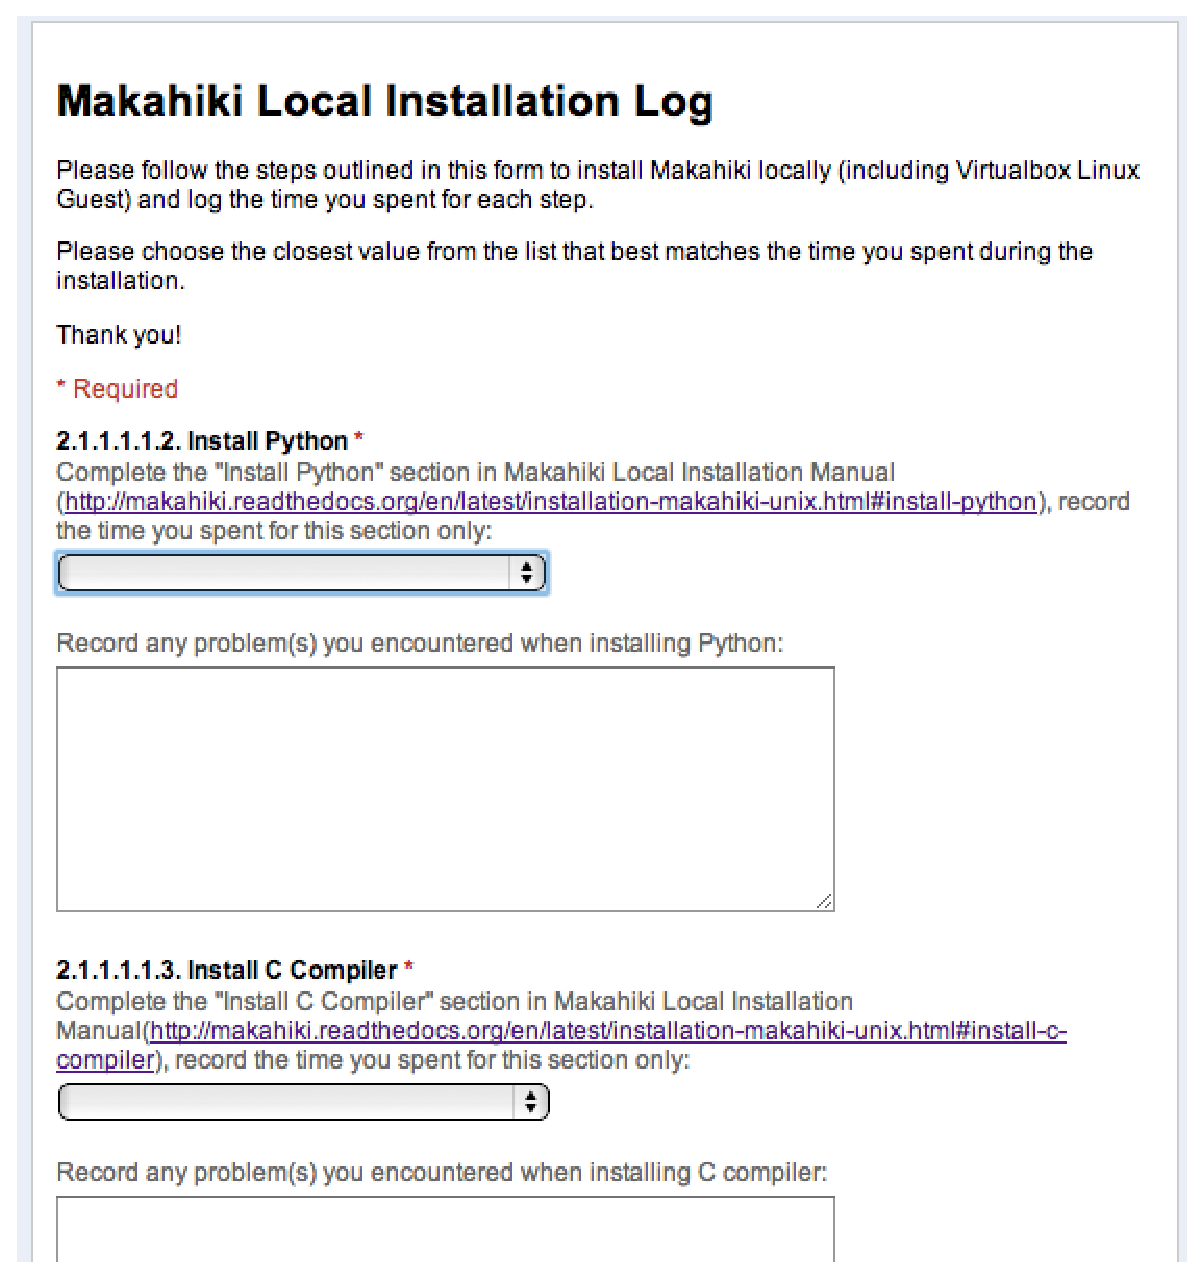
\includegraphics[height=30em,width=30em]{developer-eval-form.eps}
   \caption{Makahiki Developer assessment Form}
   \label{fig:developer-eval-form}
\end{figure}

The students will also be asked to provide feedback about their installation experiences in the form of a blog post. In the blog post, I will ask them to discuss the following topics:
\begin{itemize}
\item What is the most difficult step during installation?
\item What problems did you encounter during the installation?
\item Have you install any database, web server or similar server products prior to this assignment? Are those installations for development or production purpose?
\item If you have experience installing other servers before, How does your prior experience of installing other servers compare to the installation of Makahiki?
\item What could be improved about the Makahiki installation process?
\item Compare your experience of installing Makahiki in Heroku with installing it locally,
\end{itemize}

The data collected from the Google form responses and the blog posts from the students will be analyzed to gain insight into how easy or difficult it is to install Makahiki. 

In order to gain insight into the experience of a real world system admin who uses Makahiki, I will perform interviews to the system admin of the 2012 Hawaii Pacific University (HPU) challenge. The interview questions will include:
\begin{itemize}
 \item How much time did you spend to install the Makahiki system?
 \item How much time did you spend to maintain the Makahiki system, including backup, monitoring?
 \item What problems did you encounter during your installation and administering the Makahiki system?
\end{itemize}

I will also collect any email exchanges with the system admin regarding the installation process and maintenance of Makahiki system. Both interview and email exchange data will be analyzed to understand the system admin's experiences with Makahiki.  

\subsection{Game Designer Assessment Plan}

Similar to Makahiki system admin assessment, I plan to use two approaches to assess the game designer's experience: One is an in-lab experiment, the other is interviews with the game designers of real world Makahiki instances.

I will conduct an in-lab experiment with the same students in the ICS691 class. The students will be tasked to design a Kukui Cup-like serious game using Makahiki. I designed another Google form with the detailed steps for designing a game in Makahiki. I will ask students to follow these steps and record their time and problems encountered during their designing process. \autoref{app:googleform} has the complete Google form for the steps the students need to follow.

In addition, the students will be asked to provide feedback about their game design experiences in the form of blog posts that discuss the following topics:
\begin{itemize}
\item What is the most difficult step during Challenge Design?
\item What problems did you encounter while designing the challenge?
\item What could be improved in the Makahiki Challenge Design process?
\end{itemize}

The data collected from the responses of the game design Google forms and the blog posts from the students will be analyzed to gain insight into the game design experiences with Makahiki.

In order to gain insight into the experience of real world game designers who use Makahiki to design serious games, I will perform interviews with the real-world game designers of the 2012 Hawaii Pacific University challenge and the 2012 East West Center challenge. I will asked them about their experiences using the Makahiki game design admin interface to design their sustainability serious games. The interview questions will include:
\begin{itemize}
    \item How much time did you spend to configure the challenge global settings?
    \item How much time did you spend to design the individual games?
    \item What problems did you encounter?
    \item Did you find it difficult to design a specific game? which one, what was difficult?
    \item What did you like the least when using the system?
\end{itemize}

I will also collect any email exchanges with the game designers regarding the game design process. Both the interview and email exchange data will be analyzed to gain insight into the game design experiences with Makahiki.

\subsection{Game Manager Assessment Plan}

I plan to perform interviews with the real world game managers of the 2012 Hawaii Pacific University challenge and 2012 East West Center challenge to study the experience of game management using Makahiki. The interview questions will include:
\begin{itemize}
\item How much time did you spend to approve the action submissions?
\item How much time did you spend to monitor the game status?
\item What problems did you encounter?
\item Did you find it difficult to manage? what was difficult?
\item What did you like the least when using the system?
\end{itemize}

I will collect any email exchanges with the game managers. The data collected from the interviews and email exchanges will be analyzed to gain insight into the game managing experiences with Makahiki. 

\subsection{Developer Assessment Plan}

I plan to perform an in-lab game development study experiment with the students participating in the ICS691 serious game development class in Spring 2013. The students will be tasked with developing an enhancement to the Makahiki instance. This will involve setting up the development environment, following the tutorial to create the ``Hello world'' widget using Makahiki, and finally, developing an enhancement which extends the functionality of the Makahiki system. The enhancement is specified in 5 development tasks. 

The students will be asked to submit their development source code to the public source code repository (Github) and write a blog post to discuss their efforts in completing the development activities. The blog post should discuss the following topics:
\begin{itemize}
\item What part is complete?
\item What part is not complete?
\item Which parts you found easy or hard to complete?
\item What problems did you encounter while developing this enhancement tasks?
\item What is your recommendations for the framework to improve development support.
\end{itemize}

I will review their source code to compare their code to the reference implementation, analyze the blog posts, as well as any email correspondences regarding the problems encountered during the development. 

\section{Choose Assessment Participants}

After the assessment approaches are determined, the next step in SGSEAM is to identify the assessment participants for the different stakeholders. \autoref{table:sgseam-makahiki-participants} lists the participants for assessing the Makahiki framework using SGSEAM. 

\begin{table}[ht!]
  \centering
  \begin{tabular}{|p{0.2\columnwidth}|p{0.45\columnwidth}|p{0.2\columnwidth}|}
    \hline
    \tabhead{Stakeholder class} &
    \tabhead{Person(s)} &
    \tabhead{Organization} \\
    \hline
    Player &
    All eligible players in the UH KC instance &
    UHM \\
    \hline
    System admin &
    ICS691 students, \newline system admin for HPU instance &
    UHM, HPU\\
    \hline
    Game designer &
    ICS691 students, \newline game designers for HPU  \& EWC instance &
    UHM, HPU, EWC \\
    \hline
    Game manager &
    ICS691 students, \newline game managers for HPU \& EWC instance &
    UHM, HPU, EWC \\
    \hline
    Developer &
    ICS691 students &
    UHM\\
    \hline
  \end{tabular}
  \caption{SGSEAM Participants for Makahiki}
  \label{table:sgseam-makahiki-participants}
\end{table}

\section{Create Assessment Schedule}

After determining what the assessment approaches and who the participants are, the next step is to create the assessment 
schedule. The schedule for applying SGSEAM to Makahiki is shown in
\autoref{table:sgseam-makahiki-schedule}. 

\begin{table}[ht!]
  \centering
  \begin{tabular}{|p{0.18\columnwidth}|p{0.5\columnwidth}|p{0.18\columnwidth}|}
    \hline
    \tabhead{Time} &
    \tabhead{Task} &
    \tabhead{Assessment}  \\
    \hline
    Fall 2011 & Pre-post and in-game surveys, engagement metrics collection with UHM 2011 KC & Player experience\\
    \hline
    2012 & In-game survey, engagement metrics collection with UHM 2012 KC & Player experience\\
    \hline
    Fall 2012 & Interview with HPU KC sysadmin & System admin experience \\
    \hline
    Fall 2012 & Interview with HPU \& EWC KC game designers & Game designer experience \\
    \hline
    Fall 2012 & Interview with HPU \& EWC KC game managers & Game manager experience \\
    \hline
    Spring 2013 & In-lab installation experiment with UHM ICS691 students &  System admin experience \\
    \hline
    Spring 2013 & In-lab game design experiment with UHM ICS691 students & Game designer experience \\
    \hline
    Spring 2013 & In-lab game development experiment with UHM ICS691 students & Developer experience \\
    \hline
    Spring 2014 & in-game survey with UHM 2014 KC & Player experience \\
    \hline
  \end{tabular}
  \caption{SGSEAM Assessment Schedule for Makahiki}
  \label{table:sgseam-makahiki-schedule}
\end{table}



%% Use this for an alphabetically organized bibliography
%%\bibliography{sustainability,csdl-trs,gamification}
%%\bibliographystyle{plain}

\end{document}
